\let\negmedspace\undefined
\let\negthickspace\undefined
\documentclass[journal]{IEEEtran}
\usepackage[a5paper, margin=10mm, onecolumn]{geometry}
%\usepackage{lmodern} % Ensure lmodern is loaded for pdflatex
\usepackage{tfrupee} % Include tfrupee package

\setlength{\headheight}{1cm} % Set the height of the header box
\setlength{\headsep}{0mm}     % Set the distance between the header box and the top of the text

\usepackage{gvv-book}
\usepackage{gvv}
\usepackage{cite}
\usepackage{amsmath,amssymb,amsfonts,amsthm}
\usepackage{algorithmic}
\usepackage{graphicx}
\usepackage{textcomp}
\usepackage{xcolor}
\usepackage{txfonts}
\usepackage{listings}
\usepackage{enumitem}
\usepackage{mathtools}
\usepackage{gensymb}
\usepackage{comment}
\usepackage[breaklinks=true]{hyperref}
\usepackage{tkz-euclide} 
\usepackage{listings}
% \usepackage{gvv}                                        
\def\inputGnumericTable{}                                 
\usepackage[latin1]{inputenc}                                
\usepackage{color}                                            
\usepackage{array}                                            
\usepackage{longtable}                                       
\usepackage{calc}                                             
\usepackage{multirow}                                         
\usepackage{hhline}                                           
\usepackage{ifthen}                                           
\usepackage{lscape}
\begin{document}

\bibliographystyle{IEEEtran}
\vspace{3cm}

\title{NCERT-10.4.3.11}
\author{EE24BTECH11065 - Spoorthi yellamanchali
}
% \maketitle
% \newpage
% \bigskip
{\let\newpage\relax\maketitle}

\renewcommand{\thefigure}{\theenumi}
\renewcommand{\thetable}{\theenumi}
\setlength{\intextsep}{10pt} % Space between text and floats


\numberwithin{equation}{enumi}
\numberwithin{figure}{enumi}
\renewcommand{\thetable}{\theenumi}


\textbf{Question:}
\\
Sum of the area of two squares is 468 $m^2$. If the difference of their perimeters is 24\ $m$, find the sides of the two squares.
\\
\textbf{ Theoretical Solution: }
\\
Let the lengths of sides of the two squares be $x$ and $y$ respectively.\\
Then according to the question,
\begin{align}
    x^2 + y^2 = 468 \\
    4{\abs{x - y}} = 24
\end{align}
On squaring equation $\brak{0.2}$ on both sides, we get,
\begin{align}
    x^2 + y^2 -2xy = 36
\end{align}
On substituting equation $\brak{0.1}$ in $\brak{0.3}$, we get,
\begin{align}
    xy = 216
\end{align}
\begin{align}
    y = \frac{216}{x}
\end{align}
On substituting equation $\brak{0.5}$ in $\brak{0.2}$,
\begin{align}
    \abs{x - \frac{216}{x}} = 6
\end{align}
Case 1. $x > y$
\begin{align}
    x^2 - 6x - 216 =0
\end{align}
we get the valid value for $x$ = 18 $cm$,then y = $12 cm$\\
Case 2. $x < y$
\begin{align}
    x^2 + 6x -216 =0
\end{align}
Then $x = 12$, $y = 18$\\
$\therefore$ the lengths of sides of squares are $12 cm$ and $18cm$.\\
\textbf{Finding roots using Newton-Raphson Method:}
\\ The Newton-Raphson method is an iterative numerical technique for finding approximate solutions to equations of the form:
\begin{align}
    f\brak{x} = 0
\end{align}
It uses the equation of tangent to function.\\
we know that, for a function $f\brak{x}$, The equation of the tangent line at a point $x_n$ is given by:
\begin{align}
    y = f\brak{x_n} + f^\prime(x_n)\brak{x - x_n}
\end{align}
For the root, we set $y = 0$ (since we are looking for $f\brak{x}$ = 0, so we get:
\begin{align}
    0 = f\brak{x_n} + f^\prime(x_n)\brak{x - x_n}
\end{align}
Solving for $x$, we get,
\begin{align}
    x = x_n - \frac{f^\prime\brak{x_n}}{f\brak{x_n}}
\end{align}
This is the Newton-Raphson update formula
\begin{align}
    x_{n+1} = x_n - \frac{f^\prime\brak{x_n}}{f\brak{x_n}}
\end{align}
On choosing an initial $x_0$,and iteratively calculating the next $x$ using the update formula, we repeat the process until the difference between successive approximations is sufficiently small, i.e., until:
\begin{align}
    \abs{x - x_n} < \epsilon
\end{align}
where $\epsilon$ is a small tolerance value.\\
For our question, Let,$f\brak{x} = x^2 - 6x - 216 = 0$ (assuming $x > y$, then, 
 $f^\prime(x) = 2x - 6$\\
Then , \\
\begin{align}
    f\brak{x_n} = {x_n}^2 - 6x_n -216\\
    f^\prime(x_n) = 2x_n - 6.
\end{align}
On substituting the above expressions in the update formula,
\begin{align}
    x_{n+1} = x_n - \frac{2x_n - 6}{{x_n}^2 - 6x_n -216}
\end{align}
Let our initial guess $x_0$ = 16 and tolerance $\epsilon$ be $10^{-6}$\\
Then, we get the lengths of the sides of squares as: 18.000780944943383 and 12.000780944943383\\
\textbf{Finding roots using Bisection method:}
\\
The Bisection Method is a widely-used numerical technique for finding the roots of a continuous function. It is especially useful when you are tasked with solving equations of the form:
\begin{align}
    f\brak{x} = 0
\end{align}
where $f\brak{x}$ is a continuous function, and you are looking for the value of $x$(the root) that satisfies this equation.\\
The Bisection Method is based on the Intermediate Value Theorem, which states that if a continuous function $f\brak{x}$ changes signs between two points $a$ and $b$ i.e, $f\brak{a}.f\brak{b} < 0$, then there must exist at least one root of $f\brak{x}$ between $a$ and $b$.\\
Given an initial interval $\sbrak{a,b}$, we need to check whether $f(a).f(b)<0$, then we can compute midpoint $c$ of $\sbrak{a,b}$ as ,
\begin{align}
    c = \frac{a + b}{2}
\end{align}
if, 
\begin{align}
    f(c) = 0
\end{align}
Then the root we are looking for is $x = c$.\\
or,if
\begin{align}
    f(c).f(a) < 0
\end{align}
we can replace $b$ with $c$ and continue the process\\
if
\begin{align}
    f(c).f(b) < 0
\end{align}
we can replace $a$ with $c$ and continue the process.\\
We can iteratively keep doing this and terminate the iteration once the length of the interval becomes less than the predefined tolerance $\epsilon$.
\begin{align}
\frac{a + b}{2} - a < \epsilon \ (or) \ \frac{a + b}{2} - b < epsilon\\
    \abs{\frac{b - a}{2}} < \epsilon
\end{align}
And the root of the equation $x_0$ would become,
\begin{align}
    x_0 \approx \frac{a + b}{2}
\end{align}
In our question , on assuming the initial interval to be $\sbrak{10,20}$ and tolerance is $1e-6$,
we get the root of the equation approximately to be 17.999954223632812\\
$\therefore$ the lengths of sides of squares by bisection method are\\ 17.999954223632812 and 11.999954223632812.\\
\textbf{solution by eigen value method}
\\
If the given polynomial is 
\begin{align}
    P\brak{x} = c_0 + c_1x + c_2x^2 +..... c_{n-1}x^{n-1} + x^n
\end{align}
Then the companion matrix is given by
\begin{align}
    M = \begin{pmatrix}
        0 & 0 &....& 0 & -c_0\\
        1 & 0 & ...& 0 & -c_1\\
        0 & 1 &....& 0 & -c_2\\
        : & : & : & : &  :\\
        : & :& : & :&:\\
        :&:&:&:&:\\
        0&0&..&1& -c_{n-1}  
    \end{pmatrix}
\end{align}
And the roots of the polynomial can be found by finding the eigen values of the companion matrix.\\
For our question,
\begin{align}
    f\brak{x} = x^2 - 6x - 216
\end{align}
companion matrix is
\begin{align}
    M = \begin{pmatrix}
        0&216\\
        1&6
    \end{pmatrix}
\end{align}
The roots of the equation are the eigen values of the companion matrix.\\
We can find the eigen values by $QR$ decomposition algorithm.\\
The $QR$ algorithm is a well-known iterative procedure to compute the eigenvalues of a square matrix.\\
It decomposes a matrix $A$ into an orthogonal matrix $Q$ and an upper triangular matrix $R$ using the $QR$ decomposition and then iteratively updates the matrix by multiplying $R$ and $Q$.\\
The process continues until the matrix converges to an upper triangular form, whose diagonal elements are the eigenvalues of the matrix.\\
We start with an initial matrix $A_0 = A$, where $A$ is the matrix for which we need find the eigen values.
we take , 
\begin{align}
    A_k = Q_kR_k\\
\end{align}
$Q_k$ is an orthogonal matrix .\\
$R_k$ is an upper triangular matrix.\\
Then,next,we take
\begin{align}
    A_{k+1} = R_kQ_k
\end{align}
This new matrix $A_{k+1}$ is computed by multiplying $R_k$(from the QR decomposition) by $Q_k$.
After a sufficient number of iterations, the matrix $A_k$ will converge to an upper triangular matrix.\\
This means that the off-diagonal elements will become very small or zero, and the matrix will be nearly diagonal.\\
At this point, the eigenvalues of the matrix are located on the diagonal of the converged matrix $A_k$.\\
For our question, on taking $A_0 = M$, and applying the algorithm, we get eigen values
\begin{align}
    \lambda_1 = 18\\
    \lambda_2 = -12
\end{align}
as length of the square can not be a negative value,
the length of squares are 18 and 12 respectively.
\begin{figure}[h!]
   \centering
   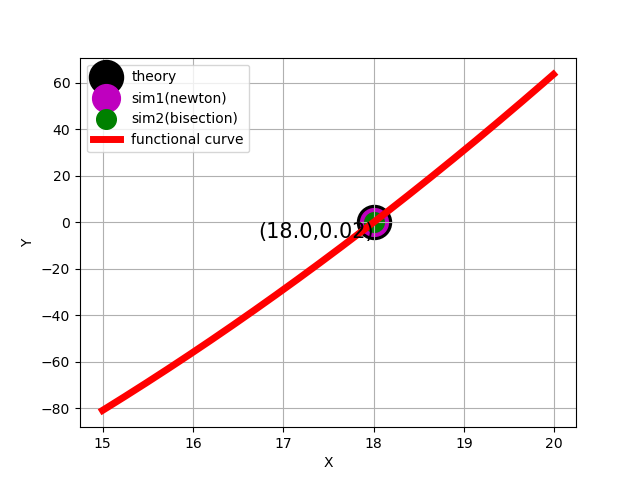
\includegraphics[width=1\columnwidth]{figures/Figure_1.png}
   \label{graph of the function}
\end{figure}


\end{document}


